\chapter{Introduction}
\label{introchap}

We stand on the threshold of a new era in robotic technology that will fundamentally change how we live and work. This robotic revolution will approach and surpass the ubiquity and usefulness of the computer revolution, because robots can change not only the virtual world, but the physical world as well. (https://h2r.cs.brown.edu/about/)

One of the main fields of research working on the expansion of these abilities to interact with the physical world is \textbf{human robot interaction} (HRI). HRI deals with the general problem of integrating robots in human populated environments. There are a number of ways in which robotics can be impactful to society in the short- mid- term. Some examples:

\begin{itemize}
    \item Hospital robots will check on patients and report their status to nurses, saving time and improving patient outcomes.
    \item Childcare robots will help parents with chores such as assisting at diaper changing or feeding, so that families can spend high-quality time together.
    \item Manufacturing robots will collaborate with people to assemble complex objects on reconfigurable assembly lines, increasing the efficiency and flexibility of factory floors.
\end{itemize}

The transition of robots from restricted access areas to human populated environments comes with a number of problems that research needs to overcome, being safety one of the key issues that needs to be addressed. Traditionally, safety in industrial robots has been achieved isolating them in a cell with safety interlocks to prevent direct interaction. HRI contributions will only be feasible once coexistence of robots and humans does not come with serious injury risk.

In order to achieve this behaviour, robots are expected to adapt to the changes in their environment. This is why it is important to study how humans interact with their environment.

Interaction between a human being and its environment is accomplished through senses. One important aspect research in robotics has focused in has been to look for ways to emulate and exploit these human senses. For example, visual sensing has been widely explored in this field. One of the reasons is the development of new low-cost depth sensors such as the Microsoft Kinect \textsuperscript{TM} has allowed to meet the many requirements of vision application at an affordable price. These depth sensors are capable of acquiring 2D images as well as the distances of the objects represented in each pixel to the camera. The usual way this data is used is to reassemble representations of obstacles in a robot-oriented space.

Other human senses are of great importance for the acquisition of data relevant to the interaction with their surroundings. Touch is one of them. Tactile sensing is the most fundamental sense when contacting the external world and it is the biggest and oldest of the sensorial organs. An experiment that consisted of exploring objects after anesthetizing the hands of a control group demonstrates that the simple task of maintaining a stable grasp of objects becomes surprisingly difficult when sense of touch is suppressed. Their hand movements are inaccurate and unstable \cite{westling1984factors}. In another experiment carried on by astronauts at the International Space Station, sense of touch was proven to be an important indicator of direction and spatial disorientation \cite{van2006touch}. Sense of touch is crucial when experiencing object properties, such as size, shape, texture and temperature. It informs about slip. It is essential to develop awareness of the body and in consequence, to differentiate one’s body from the rest of one’s surroundings. Its absence seriously hinders the interaction of an individual with its environment \cite{dahiya2009tactile}.

\begin{figure}[htbp]
    \caption[Astronauts]{
    Astronauts carrying on the experiment in ``Touch down:  the effect of artificial touch cues onorientation in microgravity''. \cite{van2006touch}
    }
    \begin{center}
    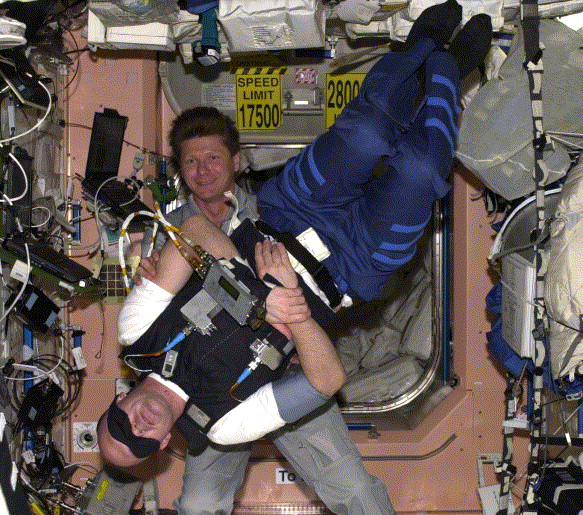
\includegraphics[width=100mm]{figs/astronauts.jpg}
    \end{center}
    \label{fig:astronauts}
\end{figure}

However, tactile sensing in robotics has not been able to achieve the penetration this evidence suggests it should have had. In traditional industrial robots, this importance has been ignored. Engineers have been able to avoid the issue of developing a artificial sensor that emulates touch by using prior knowledge about the object to be manipulated and the environment. The limitations of this approach are obvious: robots are only capable of working in structured and controlled environments. https://www.sciencedirect.com/science/article/pii/S0921889015001621

The result is that research and technology in artificial tactile sensors is not as well developed as other perception modalities. Tactile sensors in robotic applications are represented by:

\begin{itemize}
    \item\textbf{Pressure sensing arrays.} Pressure sensor matrix that provides information about the location and amount of pressure exerted on a surface.
    \item\textbf{Force-torque sensors.} They give feedback about the forces and torques that are applied on a given point in the 3 geometric axes.
    \item\textbf{Dynamic tactile sensors.} If you press your finger against an object’s corner, you can feel it for as long as you hold your finger in place. If you slowly rest your finger on the table, in contrast, you feel relatively little, until you start moving it gently back and forth. Suddenly, you are able to feel the texture, dustiness, scratches and a breadth of the properties the object has. These sensations are provided by the dynamic, fast acting tactile sensors that are embedded in the skin.
    \item\textbf{Detect changing light levels.}  https://www.wired.com/story/this-clever-robotic-finger-feels-with-light/
\end{itemize}


Current research is focused on developing tactile skins that cover robot end effectors and hands with a number of tactile sensors, in parallel with devising new algorithms that make use of these new sensors for dexterous object manipulation. However, whole body.
